% \قسمت{ارزیابی \مل{Cross-Session}}
در این بخش، نتایج ارزیابی عملکرد مدل‌ها با معیار ارزیابی \مل{Cross-Session} بررسی شده است. در این معیار، تعمیم پذیری مدل شبکهٔ عصبی در جلسات مختلف برای هر فرد بررسی می‌شود. به بیان دیگر، در این روش تعمیم پذیری شبکهٔ عصبی بین افراد مختلف مد نظر نیست اما مطلوب است که شبکهٔ عصبی با یک بار تمرین داده شدن در یک جلسه بتواند امواج مغزی همان فرد را در جلسات دیگر به خوبی طبقه‌بندی کند.

همان‌طور که گفته شد، انجام تست \مل{Cross-Validation} توسط توابع خودکار کتابخانهٔ \مل{MOABB} و با پارامترهای پیش‌فرض انجام گرفت. نتایج این ارزیابی در شکل \رجوع{میله‌ای} قابل مشاهده است. به ازای هر مقاله، دو تست اجرا شد که در یکی تنها پیش پردازش مقاله استفاده شده و خروجی آن به \مل{LDA} داده شده است و در دیگری مقاله به طور کامل تست شده است. همچنین در این شکل، عملکرد روش شناخته شدهٔ \مل{CSP+LDA} به عنوان \مل{Baseline} آمده است و یک الگوریتم طبقه‌بندی تصادفی نیز برای کمک به درک شهودی نمودار آورده شده است. در نهایت، دو روش پیشنهادی نیز از ترکیب روش‌های مختلف تولید شد که نتیجهٔ آن قابل مشاهده است.

\شروع{landscape}
\begin{figure}
\centering
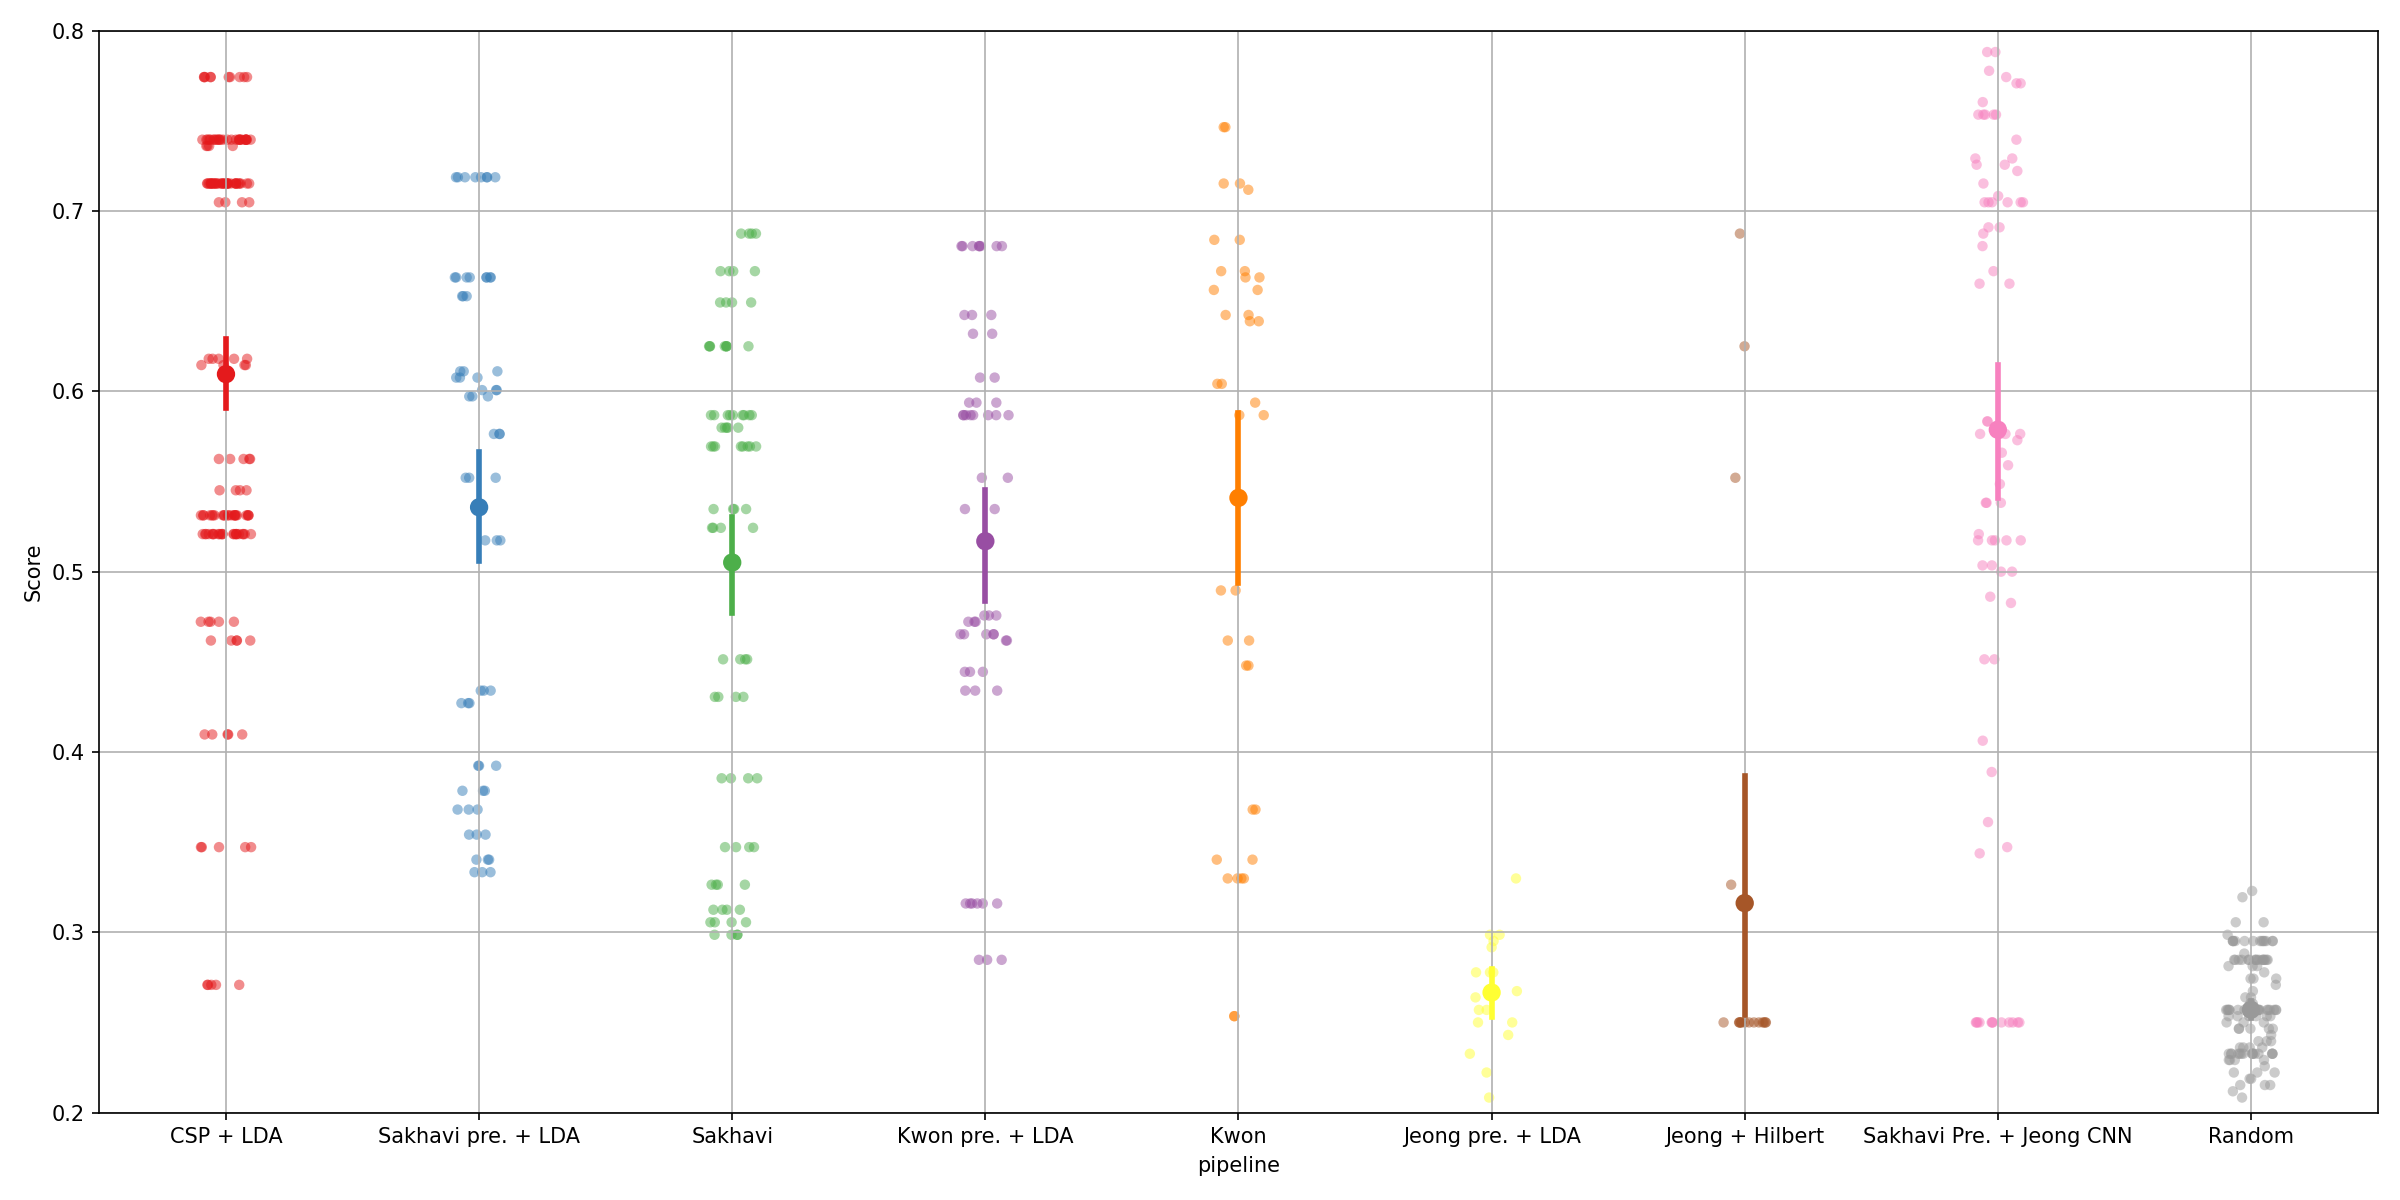
\includegraphics[width=23cm]{img/fig-bar.png}
\شرح{نمودار مقایسه‌ای امتیاز روش‌های طبقه‌بندی مختلف با معیار \مل{Cross-Session}}
\برچسب{میله‌ای}
\end{figure}
\پایان{landscape}

با توجه به شکل \رجوع{میله‌ای}، مشاهده می‌شود که روش \مل{Baseline} با برچسب \مل{CSP+LDA}، از تمام روش‌های دیگر عملکرد بهتری دارد. در بخش نتیجه‌گیری، درباره این مشاهده بحث شده است.

همچنین، مشاهده می‌شود که روش‌های پیشنهاد شده توسط \آ\ و \ب، عملکرد قابل قبولی دارند و روش \ب\ اندکی از روش \آ\ بهتر عمل کرده است به طور مشابه، ملاحظه می‌شود که روش توصیف شده در مقالهٔ \پ، خروجی ضعیفی داشته است.

از مشاهدهٔ پیش پردازش‌ها با خروجی روش‌ها این نکته جلب توجه می‌کند که در روش \آ، جداکنندهٔ خطی بهتر از شبکهٔ عصبی عمل کرده است اما در روش \ب\ شبکهٔ عصبی و جداکنندهٔ خطی عملکرد نزدیکی دارند. در روش \پ\ نیز دیده می‌شود که هم جدا کنندهٔ خطی و هم شبکهٔ عصبی هر دو عملکرد ضعیفی داشته‌اند. این مطلب که در تست‌های اولیه نیز مشاهده شد، پیشنهاد می‌داد که پیش‌پردازش استفاده شده در مدل \پ\ ممکن است عامل ضعف این شبکه باشد و باعث شد دو مدل پیشنهادی جدید با پیش پردازش‌های متفاوت اضافه شود.

در مدل اضافی اول، یک گام پردازش سیگنال به روش تبدیل هیلبرت، درست بعد از پیش پردازش و قبل از شبکهٔ عصبی مدل \پ\ اضافه شد. تبدیل هیلبرت موج‌های سینوسی حامل را حذف کرده و \مل{Envelope} سیگنال را به دست می‌آورد. به همین دلیل، در بسیاری از مواقع پردازش یک سیگنال زمانی که از آن تبدیل هیلبرت گرفته شده است، مؤثرتر می‌باشد. نتایج تست انجام شده که در شکل \رجوع{میله‌ای} نیز دیده می‌شود، پیشنهاد می‌کند که تبدیل هیلبرت در این مورد نیز می‌تواند مفید باشد.

در مدل اضافی دوم نیز پیش پردازش \آ\ با شبکهٔ عصبی \پ\ ترکیب شد و همانطور که ملاحظه می‌شود، این مورد نیز بهبود قابل توجهی را در عملکرد مدل \پ\ در پی دارد. لازم به ذکر است که پارامترهای پیش‌پردازش \آ\ به گونه‌ای تغییر داده شد که ابعاد خروجی تولید شده با ابعاد ورودی شبکهٔ عصبی \پ\ همخوانی داشته باشد.

در نهایت، نمودار رگرسیون عملکرد روش‌های منتخب، به صورت دو-به-دو در شکل \رجوع{رگ} قابل مشاهده است. با توجه به محدود بودن تعداد تست‌های موجود در دیتاست عمومی مورد استفاده، استنتاج عمومی از نمودارهای رگرسیون معتبر نخواهد بود. با این حال، این نمودارها برداشت‌های اولیه‌ای را پیشنهاد می‌دهند. به طور کلی، به نظر می‌رسد که به ازای ورودی‌های مشابه، عملکرد مدل‌ها با یکدیگر رابطهٔ مستقیم دارد. به عبارتی، هنگامی که داده‌های تمرین و اعتبارسنجی به گونه‌ای هستند که مدل الف خوب کار می‌کند، احتمال می‌رود که مدل ب نیز بهتر عمل کند و بالعکس.

\begin{figure}[h]
\centering
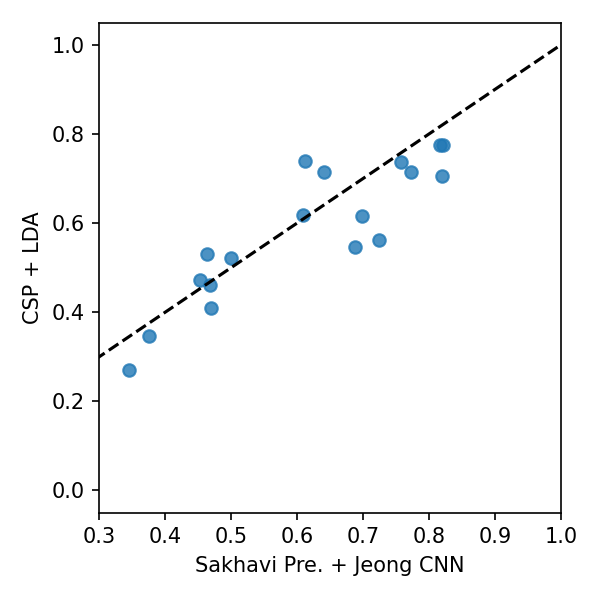
\includegraphics[width=7.5cm]{img/reg-a.png}
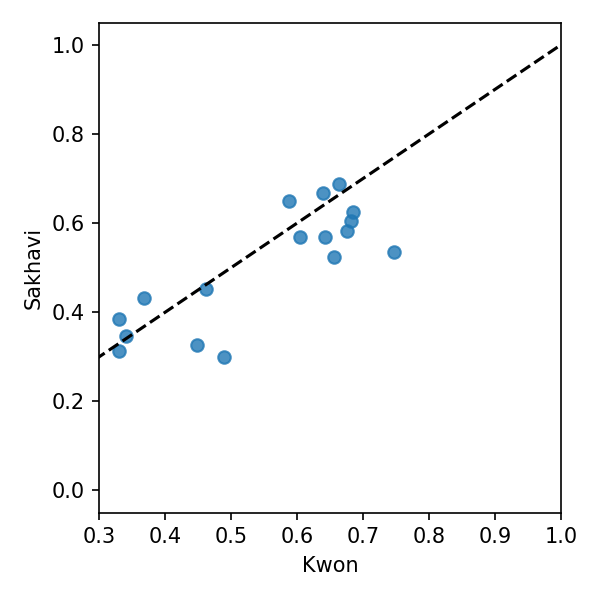
\includegraphics[width=7.5cm]{img/reg-b.png}
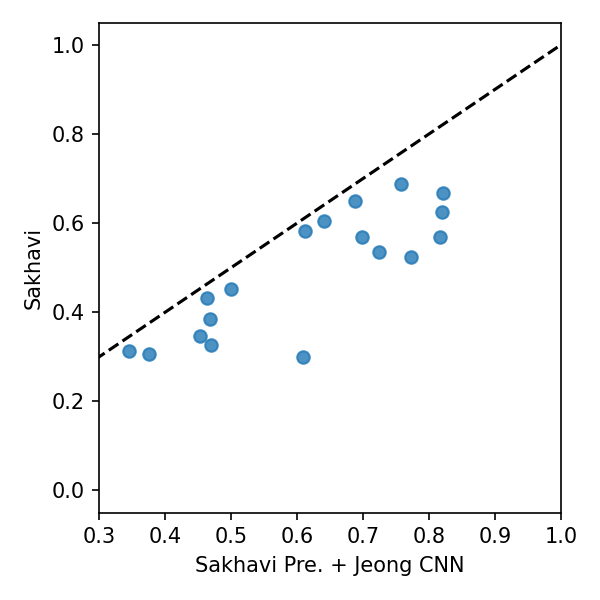
\includegraphics[width=7.5cm]{img/reg-c.png}
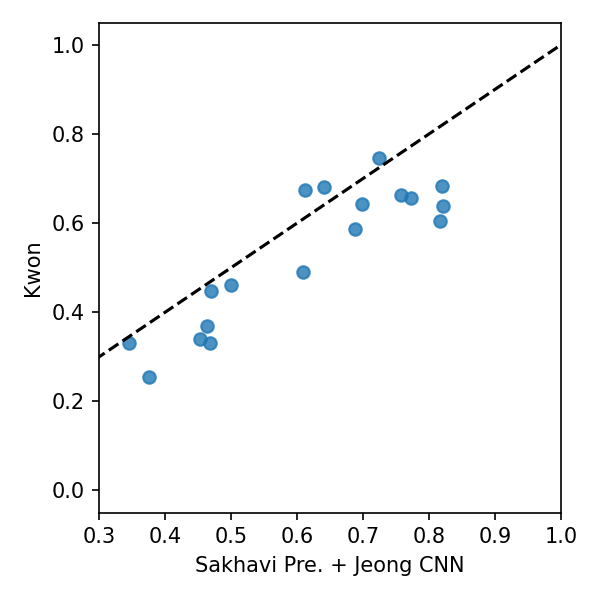
\includegraphics[width=7.5cm]{img/reg-d.png}
\شرح{نمودار همبستگی عملکردی روش‌های منتخب}
\برچسب{رگ}
\end{figure}
\begin{comment}
\begin{figure}[h]
\centering
\includegraphics[height=6cm]{img/fig-reg-1-vs-2.png}
\شرح{همبستگی امتیاز روش‌های \آ\ و \ب با معیار \مل{Cross-Session}}
\برچسب{رگ‌اول}
\end{figure}

\begin{figure}[h]
\centering
\includegraphics[height=6cm]{img/fig-reg-1-vs-3.png}
\شرح{همبستگی امتیاز روش‌های \آ\ و \پ با معیار \مل{Cross-Session}}
\end{figure}

\begin{figure}[h]
\centering
\includegraphics[height=6cm]{img/fig-reg-2-vs-3.png}
\شرح{همبستگی امتیاز روش‌های \ب\ و \پ با معیار \مل{Cross-Session}}
\برچسب{رگ‌آخر}
\end{figure}

\قسمت{ارزیابی \مل{Cross-Subject}}
در این روش، تعمیم پذیری مدل روی افراد مختلف بررسی می‌شود. به عبارتی، مطلوب است که یک شبکهٔ عصبی با تمرین داده شدن توسط یک یا چند فرد در یک یا چند جلسه، علاوه بر نمونه‌های جدید گرفته شده از این افراد، بتواند نمونه‌های افراد جدید را نیز به خوبی طبقه‌بندی کند.

ارزیابی عملکرد مدل توسط کتابخانهٔ \مل{MOABB} و با پارامترهای پیش‌فرض انجام گرفت. نتایج این ارزیابی در شکل \رجوع{میله‌ای۲} قابل مشاهده است.

\شروع{landscape}
\begin{figure}
\centering
\includegraphics[width=16cm]{img/fig-bar--2.png}
\شرح{امتیاز روش‌های طبقه‌بندی مختلف با معیار \مل{Cross-Subject}}
\برچسب{میله‌ای۲}
\end{figure}
\پایان{landscape}

همان‌طور که دیده می‌شود، الگوی عملکرد مدل‌ها در حالت \مل{Cross-Subject} به طور کلی مشابه عملکرد آن‌ها در حالت \مل{Cross-Session} می‌باشد. با این حال، با مقایسهٔ نمودار \رجوع{میله‌ای۲} با \رجوع{میله‌ای}، چند تفاوت مهم به چشم می‌خورد.

نخستین تفاوت این است که حدود نمرات تمام مدل‌ها در حالت \مل{Cross-Subject} بسیار پایین‌تر از حالت \مل{Cross-Session} می‌باشد که این مورد به دلیل این است که تفاوت‌های فردی در الگوهای امواج مغزی برداشت شده به روش \مل{EEG} نقش مهمی دارند.

تفاوت دوم این است که مشاهده می‌شود که عملکرد نسبی روش‌های مبتنی بر شبکهٔ عصبی در حالت \مل{Cross-Subject} بهتر شده است. دلیل این امر این است که در حالت \مل{Cross-Subject}، شبکه‌های مذکور با داده‌های بیشتری تمرین داده می‌شوند که عملکرد بهتر آن‌ها را در پی دارد.

همچنین، نمودارهای رگرسیون عملکرد در شکل‌های \رجوع{رگ‌اول۲} تا \رجوع{رگ‌آخر۲} قابل مشاهده است. الگوی قابل مشاهده در این شکل‌ها مشابه الگوی قابل مشاهده در تست \مل{Cross-Session} می‌باشد.

\begin{figure}[h]
\centering
\includegraphics[height=6cm]{img/fig-reg-1-vs-2--2.png}
\شرح{همبستگی امتیاز روش‌های \آ و \ب با معیار \مل{Cross-Subject}}
\برچسب{رگ‌اول۲}
\end{figure}

\begin{figure}[h]
\centering
\includegraphics[height=6cm]{img/fig-reg-1-vs-3--2.png}
\شرح{همبستگی امتیاز روش‌های \آ و \پ با معیار \مل{Cross-Subject}}
\end{figure}

\begin{figure}[h]
\centering
\includegraphics[height=6cm]{img/fig-reg-2-vs-3--2.png}
\شرح{همبستگی امتیاز روش‌های \ب و \پ با معیار \مل{Cross-Subject}}
\برچسب{رگ‌آخر۲}
\end{figure}

\end{comment}
